\refstepcounter{syllabuslesson}
\label{cur:single-winner-voting-rules}
\section{Single-Winner Voting Rules and Elections\hyperref[syllabus]{↑}}

This lesson covers criteria for evaluating single-winner voting rules, in a more technical discussions of voting methods.  This provides students a framework with which to analyze a voting method proposal.  The lesson does not go into strong and weak criteria, although that's a possibility if there is time.

In this lesson, we contrast the single-winner rules with Maryland's multi-member district Delegate elections, which use MNTV.  This aims to compare MNTV to plurality, with all the implications that has for representation in the House of Delegates.

\begin{boxcomment}
    Multi-member districts were originally used for voter suppression, and there have been calls to switch to single-member districts.  The next lesson examines single transferable vote, which provides greater representation for minority groups than single-member districts, where they can be diluted even in a Condorcet system.  This is another way for the students to draw incorrect conclusions based on incomplete knowledge, and then re-evaluate with more complete knowledge, which might drive home the point of Bayes's Theorem.
\end{boxcomment}

\subsection{Assigned Reading}

\begin{itemize}
    \item Chapter 14 of the Handbook of Social Choice and Voting \autocite[237-260]{Heckelman2015}

    \item Chapter 15 of the Handbook of Social Choice and Voting \autocite[263-281]{Heckelman2015}

    \item Four Condorcet-Hare Hybrid Methods \autocite{GreenArmytage2011}
\end{itemize}

\begin{boxcomment}
    There's a piece by Chamberlin, Cohen, and Coombs published in 1984 that I've yet to dig up for the following quote:

    ``The most striking result is the difference between the manipulability of the Hare system and the other systems. Because the Hare system considers only `current' first preferences, it appears to be extremely difficult to manipulate. To be successful, a coalition must usually throw enough support to losing candidates to eliminate the sincere winner (the winner when no preferences are misrepresented) at an early stage, but still leave an agreed upon candidate with sufficient first-place strength to win. This turns out to be quite difficult to do.

    ``One other factor also distinguishes the Hare system from the other. The strategy by which Hare can be manipulated, on the occasions when this is possible, is quite complicated in comparison with the strategies for the other methods.''
\end{boxcomment}

\subsection{Overview}

Discussions will center around the systems and criteria shown in \prettyref{fig:single-winner-criteria}.


\begin{figure}[t]
    \centering
    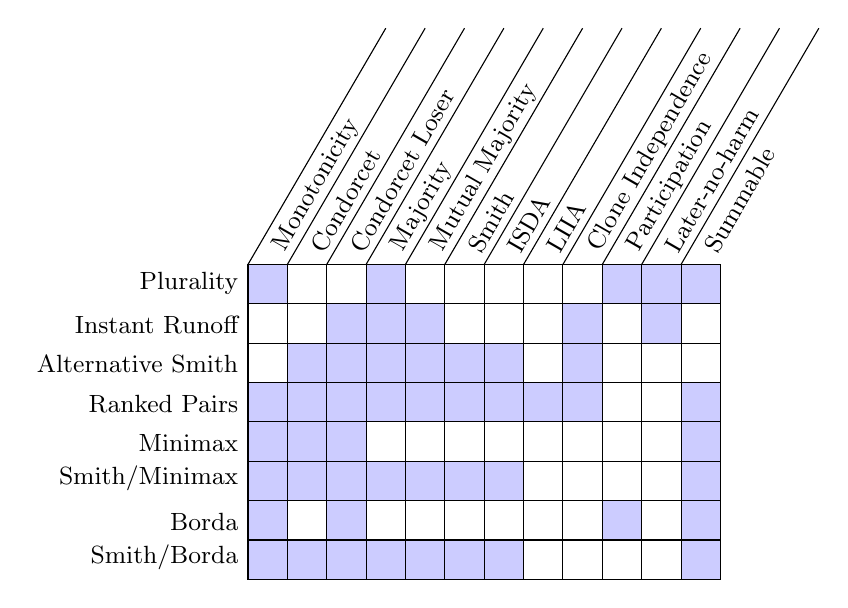
\begin{tikzpicture}[
        %sibling distance=10em,
        font=\small,
        ]
%        \foreach \x / \y in {
%            0/2,
%            1/3,
%            2/3,
%            3/4,
%            4/4,
%            5/5,
%            6/6,
%            7/7,
%            8/4,
%            9/7
%        }
%        {
%            \draw [fill=green] (\x/2,1-\y/2) rectangle ++(0.5,-0.5);
%        }
        \foreach \x / \y in {
            0/0, 3/0, 9/0, 10/0, 11/0, % Plurality
            2/1, 3/1, 4/1, 8/1, 10/1, % IRV
            1/2, 2/2, 3/2, 4/2, 5/2, 6/2, 8/2, % Alternative Smith
            0/3, 1/3, 2/3, 3/3, 4/3, 5/3, 6/3, 7/3, 8/3, 11/3, % Ranked Pairs
            0/4, 1/4, 2/4, 11/4, % Minimax
            0/5, 1/5, 2/5, 3/5, 4/5, 5/5, 6/5, 11/5, % Smith/Minimax
            0/6, 2/6, 9/6, 11/6, % Borda
            0/7, 1/7, 2/7, 3/7, 4/7, 5/7, 6/7, 11/7 % Smith/Borda
        }
        {
            \draw [fill=blue!20] (\x/2,0-\y/2) rectangle ++(0.5,-0.5);
        }
        \foreach \x[count=\xi] in {
            Monotonicity,
            Condorcet,
            Condorcet Loser,
            Majority,
            Mutual Majority,
            Smith,
            ISDA,
            LIIA,
            Clone Independence,
            Participation,
            Later-no-harm,
            Summable
        }
        {
            \node at (0.5*\xi-0.35,0) [anchor=south west] {\rotatebox{60}{\x}};
            \draw (0.5*\xi-0.5,0) -- ++(1.75,3);
            \draw (0.5*\xi-0.5,0) -- ++(0,-9/2+0.5);
        }

        \draw (0,0) -| ++(6,-4);
        \foreach \x[count=\xi] in {
            Plurality,
            Instant Runoff,
            Alternative Smith,
            Ranked Pairs,
            Minimax,
            {Smith/Minimax},
            Borda,
            Smith/Borda
        }
        {
            \node at (0,-0.5*\xi) [anchor=south east] {\x};
            \draw (0,-0.5*\xi) -- (6,-0.5*\xi);
        }

    \end{tikzpicture}
    \caption{\label{fig:single-winner-criteria}Single-winner voting rule criteria.}
\end{figure}

\begin{itemize}
    \item Begin by discussing that different voting rules—the rules about how ballots will be counted and the winner selected—have different properties affecting whose vote matters and how representative the election is.
    \begin{itemize}
        \item Recalling \hyperref[cur:majority]{the lesson on majorities}, discuss plurality versus pairwise majorities, and the behavior we've seen in instant runoff voting.
    \end{itemize}

    \item Address various criterion by examining and discussing individual rules
    \begin{itemize}
        \item Use Alternative Smith to demonstrate constriction of a voting rule to the Smith set

        \item Use Ranked Pairs and Minimax to demonstrate summability
        \begin{itemize}
            \item Summability allows us to count ballots in subsets and then add the results together

            \item Counts can be observed at the place and time of voting, maintaining integrity

            \item Counts can be added along the way, allowing continuous reporting of results as with plurality
        \end{itemize}

        \item Discuss, particularly, the perceived versus actual value of later-no-harm and participation

        \item Discuss the difference between logical failure (a rule is not mathematically immune to failing a criterion) and probable failure (a rule may fail a criterion in rare cases, or only in contrived examples)
    \end{itemize}

    \item Address primary election cycles
    \begin{itemize}
        \item With too many candidates, voters can't become informed enough to provide a sufficient number of rankings
        \begin{itemize}
            \item Many ballots don't rank the candidate who would be the Condorcet winner if all voters were as informed about all candidates as they are about their favorite \textit{and} ranked their preferences for all candidates

            \item This often results in an outcome identical to if the plurality coalition were the only voters
        \end{itemize}

        \item Discuss party primary with various rules
        \begin{itemize}
            \item Party primary excludes subsets of voters, which—as in our IRV example—allows a specific set of voters to remove choices before other voters can vote.  Compare this to serial dictatorship, where if the dictator doesn't vote, then the second dictator votes; and if the second dictator doesn't, then the third; and so forth.

            \item Plurality and Condorcet both have major flaws under party primary, due to exclusion of voters
        \end{itemize}

        \item Discuss Top-Two and Final-Five primary elections
        \begin{itemize}
            \item Both select the top several candidates with the most votes

            \item Consider ranking and Condorcet instead, removing the Condorcet winner and then identifying the new Condorcet winner until having selected enough:  with too many candidates, we can't rely on voters to rank enough to select the Condorcet winner, and you get a series of candidates all representative of a plurality group of voters

            \item Top-two can lock out the majority

            \item Final Five is less prone to majority lockout, but can be affected by vote splitting as can plurality
        \end{itemize}
    \end{itemize}

    \item Address total election cycles
    \begin{itemize}
        \item Party primary with instant runoff voting is functionally just party primary and then a vote between just the two party nominees; see Burlington, VT, 2009 Mayoral Election for three strong parties

        \item Top-Two's lock-out need not be discussed because top-two always comes down to a single pairwise election

        \item Final Five uses instant runoff as its general election; the class discussion should eventually discuss a summable Condorcet method like Ranked Pairs or Smith/Minimax
    \end{itemize}

    \item Address the Maryland House of Delegates election
    \begin{itemize}
        \item This elects multiple members

        \item Voters get one vote per Delegate to be elected

        \item Vote totals are used to elect the top 3 delegates

        \item This tends to allow a plurality of voters to control all three
    \end{itemize}
\end{itemize}

\subsection{Criteria}
\begin{todo}
    Better explanations.
\end{todo}

\begin{boxcomment}
    Do not test students on relative weakness of criterion.  This is a ridiculous thing to try to memorize and is barely useful even when doing mathematical analysis of voting rules, much less in an introductory course on philosophy and basic election mechanics.
\end{boxcomment}

\begin{definition}{Weakness}
    A voting criterion is ``weaker'' than any criterion by which it is implied.
\end{definition}

Weak criterion imply strong criterion.

\begin{itemize}
    \item Majority criterion (MC) is weaker than mutual majority (MMC) because a simple majority is also a mutual majority, and when no simple majority exists a rule satisfying MC need not elect from the mutual majority.

    \item Condorcet is weaker than mutual majority, because a Condorcet method need not elect from the mutual majority set when there is no unique Smith candidate.

    \item Mutual majority is weaker than Smith, as the Smith set is a subset of the mutual majority set.

    \item Condorcet (winner) and Condorcet loser are weaker than Smith.

    \item Local independence of irrelevant alternatives (LIIA) is weaker than IIA.

    \item Smith is weaker than independence of Smith-dominated alternatives (ISDA) because a rule electing from the Smith set may be influenced by non-Smith candidates (e.g. Nanson, Baldwin).

\end{itemize}

\begin{definition}{Independence of Irrelevant Alternatives}
    The group's preference between candidates $X$ and $Y$ is determined only by the individual preferences between $X$ and $Y$.
\end{definition}

Independence of Irrelevant Alternatives (IIA) is practically impossible to satisfy.  Approval and Score theoretically satisfy IIA if voters mark each candidate on their ballot as if they don't know of the existence of any other candidate; this is patently absurd, as whether a voter approves of a candidate or how high a score they receive is dependent on the other candidates available.

Approval reduces to plurality when candidates are diverse and match voter ideals:  voters approving only candidates roughly similar to some degree will not approve other candidates.  Broken into three or more core coalitions, the largest coalition selects the winner.  When all voters approve all but the least-liked candidate, the system is equivalent to anti-plurality.

There is no absolute measure of welfare, so the highest-scored candidate from 0 to 1 must be scored 1.0 to make logical sense.  Score's claim to IIA requires voters to not exercise full voting power; more than that, it requires an absolute scale of welfare applied correctly by all voters, by which the highest possible welfare is 1.0 and the lowest is 0.  These theoretical explanations are nonsense.

\begin{definition}{Local Independence of Irrelevant Alternatives}
    If some subset of alternatives in consecutive positions of win order is selected and all other alternatives deleted from all votes, the win order of the subset must remain unchanged.
\end{definition}

LIIA requires that if the winner is rendered unranked on all ballots, the second-place winner will win; and if the loser is rendered unranked, the second-place loser will become the last-place loser.  Few methods satisfy LIIA, notably Ranked Pairs; Kemeny-Young can become technically impossible to calculate for some candidate sets as it is NP-Hard.

Plurality fails LIIA because it simply discards all but the first rank.  Theoretically, voters have unexpressed preferences due to the ballot being single-mark.  Instant runoff voting demonstrates plurality with repeated elimination of the loser:  the plurality winner in one round is not always the plurality winner in the next.  Eliminating the plurality winner on a ranked ballot can elevate the last-place candidate above the second-place candidate.

\begin{definition}{Condorcet criterion}
    A voting rule passes the Condorcet criterion if it elects the Condorcet candidate when one exists.  Also called the Condorcet winner criterion.
\end{definition}

\begin{definition}{Condorcet loser}
    A candidate for whom every opponent receives a pairwise majority of votes.
\end{definition}

\begin{definition}{Condorcet loser criterion}
    A voting rule passes the Condorcet loser criterion if it never elects the Condorcet loser when one exists.
\end{definition}

When there is no Condorcet winner, a rule may elect anyone.  Minimax always elects the Condorcet winner, but can otherwise elect any candidate including the Condorcet loser.  All runoff methods and Smith-efficient rules satisfy Condorcet loser.

\begin{definition}{Monotonicity}
    A voting rule is monotonic if raising a candidate's ranking from its original position only increases or leaves unchanged its group ranking.
\end{definition}

Instant runoff voting fails monotonicity:  when, after running off to three options, the different votes between the Condorcet candidate and a candidate outside the mutual majority is larger than the difference between the winning candidate and a simple majority, raising the winning candidate to first place on as many ballots causes the minority candidate to be eliminated before the Condorcet candidate, and the Condorcet candidate is elected.  In this condition, ranking the winning candidate higher on several ballots causes that candidate to lose.

Many Smith-efficient methods satisfy monotonicity because raising a candidate gives them a stronger position.  Geller-IRV and Geller-STV eliminate by Borda count, and so raising a candidate decreases their likelihood of elimination while raising their likelihood of having enough votes to be elected.  Smith/IRV is non-monotonic for the same reasons as IRV.  Ranked Pairs, Schulze, Split Cycle, and others are monotonic.

\begin{definition}{Participation}
    A voting rule satisfies the participation criterion if adding a ballot where Candidate $X$ is preferred to Candidate $Y$ cannot change the winner from $X$ to $Y$.
\end{definition}

\begin{definition}{Consistency}
    A voting rule satisfies the consistency criterion if two sets of ballots tabulating to identical results also produce an identical result when tabulated together as one set of ballots.
\end{definition}

Participation and consistency reduce mathematically to the same function:  each implies the other.  No known viable voting system satisfies these criterion, notably Borda because of its extreme manipulability and plurality for obvious reasons are not considered ``viable.''

\begin{definition}{Clone independence}
    A voting rule is independent of clones when adding or removing candidates to clone sets does not affect the winning chance of any candidate not in the set of clones.
\end{definition}

We can think of a clone set as a set of candidates for which no voter ranks any candidate outside the set between or equal to those inside the set, or a rough approximation there of.  This is too broad, and in practice clones must be substantially-similar, so the definition is somewhat imprecise and conceptual.

Instant runoff voting is immune to clones because it will eliminate one or the other at the same stage, transfer votes exclusively to the surviving clone, and then place the surviving clone in the original elimination order.  Ranked Pairs is similarly immune because clones have the same (or substantially similar) pairwise victories, and so their order of placement doesn't change.  Unpopular ideological clones just end up at the bottom with few votes.

Of interest:

\begin{itemize}
    \item Smith criterion implies Condorcet and Mutual Majority.

    \item Condorcet implies Majority Winner, but does not imply Mutual Majority.

    \item Mutual Majority implies Majority Winner and Majority Loser, but not Condorcet Loser (Bucklin satisfies Mutual Majority but not Condorcet Loser).

    \item Smith is incompatible with later-no-harm, favorite betrayal, participation, and consistency, and independence of irrelevant alternatives.

    \item Any voting rule constricted to the Smith set by treating as withdrawn all non-Smith candidates is independent of Smith-dominated alternatives (ISDA); otherwise they may not be ISDA.  Nanson's and Baldwin's methods satisfy Smith, but not ISDA.
\end{itemize}

Single-winner methods and evaluation criteria
\begin{itemize}
    \item Plurality
    \begin{itemize}
        \item Satisfies
        \begin{itemize}
            \item Monotonic:  More voters voting for X can't make Y more likely to win

            \item Majority:  If there is a first-order winner, they are elected (silly criteria…)
        \end{itemize}
        \item Fails
        \begin{itemize}
            \item Clone independence:  Adding a candidate exactly as preferred by all voters as another can't change the outcome (plurality suffers vote splitting)
            \item Condorcet:  Elects the condorcet winner (Plurality doesn't even check)
            \item Majority loser:  can't elect the majority loser.  (Plurality can elect a candidate for whom a majority of voters prefers EVERY OTHER CANDIDATE over them, i.e. not just loses to everyone, but loses spectacularly)
            \item Condorcet loser:  a stronger version of Majority loser, where a candidate is preferred by some majority of voters to each other candidate, but not necessarily by a single majority to all other candidates.  (Fails this hard)
        \end{itemize}
    \end{itemize}
    \item Instant Runoff Voting
    \begin{itemize}
        \item Satisfies
        \begin{itemize}
            \item Majority:  the winner has to have a majority of votes over at least 1 other candidate (showing how useless Majority is)
            \item Mutual majority:  If a majority of voters exists whose top n preferences are the same, but in different orders, the majority with the smallest value n is the mutual majority, and the candidates in question are the mutual majority set.  The winner must be one of these.  (This paired with later-no-harm causes a severe error in IRV)
            \item …Thus Condorcet loser and Majority Loser.
            \item Later-no-harm:  if a voter ranks an additional candidate as less-preferred than all other candidates, doing so doesn't cause one of their higher-ranked candidates to lose
            \item Later-no-help:  if a voter adds a candidate as in later-no-harm, doing so doesn't cause one of their higher-ranked candidates to win.
            \item Clone independence
        \end{itemize}
        \item Fails
        \begin{itemize}
            \item Participation:  a voter can't get a better result by not voting.  (This failure is demonstrated in the first class.  Tactically, the voter is better off voting for the better result they think they will get by not voting, and their favorite second)
            \item Favorite betrayal:  a voter can't make their favorite win by ranking someone above their favorite.  (Under IRV, voting for candidate X can cause Y to be eliminated before candidate A, transferring votes to A.  This may cause A to win, whereas the same voter voting for A first can cause A to lose.)
            \item Monotonic
            \item Condorcet
        \end{itemize}
    \end{itemize}
    \item Minimax
    \begin{itemize}
        \item Satisfies
        \begin{itemize}
            \item Monotonic
            \item Condorcet
            \item Majority
            \item Summable (only need the pairwise results, so ballot counting can be divided up)
        \end{itemize}
        \item Fails
        \begin{itemize}
            \item Majority loser (implying it fails Condorcet, Mutual Majority.  Minimax can elect any candidate.)
            \item Smith:  if no Condorcet winner exists, selects from the smallest set where any single one of these would be the Condorcet winner if the others were removed.  (Failing Majority Loser, Condorcet, Mutual Majority all imply failing this)
            \item Clone independence
            \item Participation
            \item Later-no-harm/help
        \end{itemize}
    \end{itemize}

    \item Ranked Pairs
    \begin{itemize}
        \item Satisfies
        \begin{itemize}
            \item Monotonic
            \item Condorcet
            \item Majority
            \item Mutual majority
            \item Clone independence
            \item Smith
            \item Independence of smith-dominated alternatives:  candidates not in the Smith set have no effect on the outcome
            \item Local independence of irrelevant alternatives:  Deleting the last-place winner must not change the outcome; deleting the first-place winner must cause the second-place winner to be elected
            \item Summable
        \end{itemize}

        \item Fails
        \begin{itemize}
            \item Participation
            \item Later-no-harm/help
        \end{itemize}
    \end{itemize}
\end{itemize}

\subsubsection{Range Voting}

A note on range voting.

The Range Voting Web site indicates Arrow's is violated by score voting systems, but that can be proven untrue.  It's only independent of irrelevant alternatives if voters don't change their other scores, which assumes voters don't use full voting power.  Whenever a candidate is introduced who any voter prefers more than their otherwise first-choice candidate, that first-choice candidate is either scored less than the maximum (not exercising full voting power) or all scores are adjusted to fit the new top-scored candidate.  Whether other candidate scores are altered equally, unequally, or in proportion, there is a scenario where a winning candidate becomes a loser and a losing candidate becomes a winner as a result of this new losing candidate.

All Condorcet methods are independent of irrelevant alternatives when there is a Condorcet winner.  That's not the point.

\url{https://www.princeton.edu/~cuff/voting/theory.html} hits this point.

Given the possibility that any single voter may exist whose preferences are the same as their scores, with higher scores being higher preference, the conditions given to satisfy IIA cannot be satisfied.  A voter may have three candidates $\left\{A,B,C\right\}$ such as to rate $A=1.0$ and both $B=0.0$ and $C=0.0$; to elevate $C$ above $A$, the voter must reduce the ranking of $A$.  No matter how small this reduction, the margin between $A$ and $B$ can be so small as to be smaller, and so the winner changes from $A$ to $B$; and even in a finite field where movements are not infinitely small, $A$ can become tied with $B$.  This single example shows a violation of one criterion which Arrow's Impossibility Theorem says can never be simultaneously true along with non-dictatorship and Pareto.